% mainfile: ../praca_magisterska_orbifoldy.tex
\chapter{Algorithm for searching for the spectrum}\label{Searching the spectrum}

In the previous chapter we answered the questions about how $\spe$ looks like -- in particular 
what is it's order type and topology. In this chapter we would like to develop a 
methods for answering the 
following question: 
%In the previous chapter the main question was about which rational numbers are in $\spe$. 
%We can ask, how to answear the question 

%In this chapter we will show that the question 
"For a given rational number, is it in $\spe$?" 

We have some sort of answer to this question -- an algorithm.
%a very long equation that 
%commonly is refered to as an algorithm. 

It is not an ideal answer as it gives little insight of what is a general structure 
of the spectrum. Nevertheless it is a constructive and computable answer. 
%What's more, 
%later, in implementation chapter we discuss that for numbers with denominators of a reasonable 
%size and in reasonable distance from zero this algorithm can be run successfully on a 
%personal computer.

%is computable.

%In this chapter, we will provide the best answear we could find. 

%Turns aout that the number is in the specturm iff the following procedute says "yes". 

%It turns aout that the question for any number is answearable  

%Algorithmical approunch to questions from chapter 3 are only possible after gfiniteness 
%part of chapter four.

%What we can show, is that this question is computable -- i.e. there exists an algorithm 
%that answears this question. 

%Using results from previous chapters, we can now prove, that some computational problems related 
%to spectra are solvable.

%We will do it in a constructive way, by writing explicitly the algorithm and proving its
%correctness.

% and properties.

%We will also be able to actually compute sufficiently small examples of the 
%question.
%unansweared question 

The exact question we will provide algorithm to answer here is: 

\textit{For a given rational number $r$ and manifold $M$, is there at least one 
$M$ orbifold with $r$ as its \Eoc?}

%For a given rational number $r$ and manifold $M$:
%\begin{itemize}
%\item How many $M$ orbifolds with $r$ as their \Eoc\ are there?
%\item The accumulation point of what degree is $r$ in $\spe(M)$?
%\end{itemize}

We start with $r=\frac{p}{q}$, where $p \in \mathbb{Z}$, $q \in \mathbb{N}_{>0}$ and a manifold $M$. 
%\section{Reductions and special cases}

%\section{Decidability}
%\todo{oj dokończyć}
%Here we will show the proof that the problem of "deciding whether a given rational number is in an 
%Euler orbicharacteristic's spectrum or not" is decidable by showing algorithm for doing this. 
%Later, our algorithm will have a bonus property of determining of which order of condensation 
%is given point if it is in fact in $\sigma$. \\
%\smalltodoII{Może od razu postawić pełny problem}
%%It fill get also a performance enhancement by this added property. \\
%First stated algorithm is also very inefficient and is presented, because the idea is the most 
%clear in it. Right after it there is stated an algorithm with two enhancements: 
%\begin{itemize}
%\item determining an accumulation point of which order is a given point, if it is in fact in the 
%spectrum (this enhancement gives also a performance boost) 
%\item faster searching, because some cases do not need to be checked. 
%\end{itemize}
%\subsection{The algorithm}
%and $\textrm{gcd}(p,q)$. \\ 
\section{Reduction from arbitrary $M$ to $D^2$}\label{algorithm reduction to D2}
This reduction is based on \ref{spe_M}.
Note, that this is a different reduction than the one in chapter \ref{reduction_to_arithmetical}. 
In chapter \ref{reduction_to_arithmetical} we are saying that for any $M$, we have $\spebr{M} 
\subseteq \speS \cup \speD$. In \ref{spe_M} on the other hand we have, that 
for a manifold $M$ with $h$ handles, $c$ crosscaps and $b$ boundary components: \\
for $b \neq 0$:
\begin{equation}
\spe(M) = \speD + \chi(M) -1 = \speD - 2h - c - (b - 1)
\end{equation}
and for $b = 0$:
\begin{equation}
\spe(M) = 2\speD + \chi(M) - 2 = 2\speD - 2h - c.
\end{equation}  


%Using \ref{spe_M} 
%and \ref{} 
We conclude that the problem of deciding whether $\frac{p}{q}$ is in $\spe(M)$
is equivalent to deciding: \\
for $b \neq 0$ if:
\begin{equation}\label{translation with b not 0}
\frac{p}{q} - \chi(M) + 1 = \frac{p}{q} + 2h + c + (b-1) 
\end{equation} 
is in $\sdD$; \\
for $b = 0$ if:
\begin{equation}\label{translation with b 0}
\frac{1}{2}\frac{p}{q} + \chi(M) + 2 = \frac{1}{2}\frac{p}{q}+h+\frac{c}{2}
\end{equation}
is in $\sdD$.

Considering this fact, from this point, WLOG we will assume that $M = D^2$ and, 
following \ref{only dihedral}, we will 
be concerned only with dihedral orbipoints.

%\subsection{Arithmetic formulation}
%We want to determine whether there exists $d_1,d_2,\cdots,d_k$, such that 
%$\chi^{orb}(*d_1\cdots d_k) = \frac{p}{q}$. 

\section{Special cases}
In the case that $\frac{p}{q}$ is of the form $l\frac{1}{4}$, for some $l \in \mathbb{Z}$ 
% $q = 4$ 
we can give the answer right away. For $l > 4$ we have that $l\frac{1}{4}$ is not in the set 
and for $l \leq 4$ it is (see \ref{greatest \apots}). 

Moreover for an even $l$ we have that $l\frac{1}{4}$ is an accumultion point of order 
$\frac{4-l}{2}$ 
and for an odd $l$ it is an accumulation point of order $\frac{3-l}{2}$ (see \ref{greatest \apots} 
and \ref{predescors}). 

In the case, where $\frac{p}{q} > 1$, we also can give answer right away and this answer is "no". 

Now we will consider only cases when $\frac{p}{q}$ is not of the form $l\frac{1}{4}$ and is 
$\leq 1$.
%\section{General case}
%
%\section{Simpler version of the question}
%
%To present the idea of searching the spectrum for the orbifolds with a given \Eoc, we will 
%first present the algorithm that answears a little easier question, namely: 
%
%\textit{For a given rational number $r$ and manifold $M$, is there at least one 
%$M$ orbifold with $r$ as their \Eoc?}
%
%This algorithm will mirror what we are focused on in \ref{chapter_three}, giving us the 
%computational tool for deciding whether a given number is in the spectrum or no. 
%
%The first approach of the searching algorithm is of this form: \\
%
%%We start with the 
%We use: 
%\begin{itemize}
%$\mathbb{N}$ counters $d_1d_2\cdots$ 
%(with values ranging from $1$, through all natural numbers, to infinity 
%(with infinity included)) set to $1$. Each counter correspond to one cone point 
%on the boundry of the disk of period equal to the value of the counter (with the note, that 
%if counter is set to $1$ it means a trivial cone point - namely a none cone point, a normal 
%point). 
%Every state of the counters during runtime of the algorith will have only finitely many 
%counters with value non-$1$. Moreover every state in the rutime of the algorithm 
%will have values on consequtive counters ordered in weakly decreasing order. From now we will 
%consider only such states. \\
%The state $d_1d_2\cdots$ correspond to the orbifold of 
%\Eoc equal $\chi^{orb}(*d_1d_2\cdots)$ (where the trailing $1$ are trunkated). \\ 
%%There is also a pivot pointing on one counter at any time.  
\section{Regular cases}
First we will describe what we use in the algorithm, giving the brief semantics. 
The detailed semantics are given in \ref{the idea of the algoritm}.
\subsection{What we use}
We use: 
\begin{itemize}
\item $\mathbb{N}_{>0}$ counters $c_1, c_2, \cdots$ 
with values ranging on $\mathbb{N}_{>0}\cup\{\infty\}$.
%$1$, through all natural numbers, to infinity 
%(with infinity included). 
Each counter correspond to one dihedral point 
on the boundary of the disk of period equal to the value of the counter (with the note, that 
if counter is set to $1$ it means a trivial dihedral point - namely a non-orbi point, 
a normal point). 

We will write the state of the counters without commas, using the letter $d$. 
Note that with this convention, $c_i$ will refer to the $i$-th counter and $d_i$ will 
refer to the value of the $i$-th counter. 

So the state of the counters $d_1d_2\cdots$ correspond to the orbifold 
$*d_1d_2\cdots$ (where the trailing $1$'s are truncated).

We will refer to the counters being "to the left" or "to the right" of each other, as 
the numbering would go from left to right.

\item a pivot pointing at some counter 
% at any time
\item a flag that can be set to: "Greater", "Searching" or "Less" corresponding to what was 
the outcome of comparing \Eoc\ of the orbifold corresponding to counters' state and 
$\frac{p}{q}$ or to the fact, that there is a need for a search of the next state of counters 
to compare with $\frac{p}{q}$.  
\end{itemize}
\subsection{What state are we starting our algorithm with}
We start with:
\begin{itemize}
\item all counters set to $1$. 
\item pivot pointing at the $c_1$
\item flag set to "Greater"
\end{itemize}
%If $\frac{p}{q}$ is of form $\frac{k}{4}$, where $k \in (-\infty,8] \cap \mathbb{Z}$ we give 
%the answear "yes" and end the whole algorithm. If $\frac{p}{q} > 2$ we give the answear "no" and 
%end the whole algorithmBecauseof this, below we assume, that \\
\subsection{Invariants claims}
Now we will state the claims of what properties the state of the counters will maintain 
during all the execution of the algorithm. The proof, that this is indeed the case will 
be performed in 
\ref{memory state proof}
\begin{claim}\label{valid state of counters}
We will do our computation such that:
\begin{itemize}
\item every state of the counters during runtime of the algorithm will have only finitely many 
counters with value non-$1$. 
\item every state in the runtime of the algorithm 
will have values on consecutive counters ordered in weakly decreasing order.
\end{itemize}
\end{claim}
From now we will 
consider only such states. 

%There is also a pivot pointing on one counter at any time.  
%The state of the counters $d_1d_2\cdots$ correspond to the orbifold 
%%of \Eoc\ equal $\chi^{orb}(*d_1d_2\cdots)$
%$*d_1d_2\cdots$ (where the trailing $1$'s are trunkated). 
\subsection{The algorithm for searching for a spectrum}
\label{the algorithm for searching the spectrum itself}
When the algorithm is in the state: 
\begin{itemize}
\item counters with values: $d_1d_2\cdots$
\item pivot: at the counter $c_p$
\item flag: set to the value $flag\_value$,
\end{itemize}
we proceed as follows 
%(the term "We continue." means, that we start the following procedure from the beginning)
:
%// More on how we search for it will be told later, 
%        // for now we can think that we search one by one,
%        // starting from $d_p$ and going up till $d_p'$.
\begin{lstlisting}[firstnumber=1,consecutivenumbers=true]
In the case, the $flag\_value$ is equal to: 
{
    "Greater", then
    {
        If $\chi^{orb}(*d_1\cdots d_{p-1}\infty d_{p+1}\cdots)=\frac{p}{q}$ then
        {
            We found an orbifold and we are ending the whole
            algorithm with answer "yes, $*d_1\cdots d_{p-1}\infty d_{p+1}\cdots$".
            
            
            
        } 
        If $\chi^{orb}(*d_1\cdots d_{p-1}\infty d_{p+1}\cdots)>\frac{p}{q}$ then
        {
            We set $d_p$ to $\infty$.
            We set the flag to "Greater".
            We put the pivot at the $c_{p+1}$.
            We go to the 1st line.
        }  
        If $\chi^{orb}(*d_1\cdots d_{p-1}\infty d_{p+1}\cdots)<\frac{p}{q}$ then
        {
            We set the flag to "Searching".
            We go to the 1st line.
        }  
    }
    
    "Searching", then
    {
        We search one by one 
        for the value $d_p'$ of the $c_p$ such that
        $\chi^{orb}(*d_1\cdots d_{p-1}d_p'd_{p+1}\cdots)\leq\frac{p}{q}$ and
        $\chi^{orb}(*d_1\cdots d_{p-1}(d_p'-1)d_{p+1}\cdots)>\frac{p}{q}$.
        We set $c_p$ and all of the counters 
        to the left of $c_p$ to the value $d_p'$.
        if $\chi^{orb}(*d_1d_2d_3\cdots)=\frac{p}{q}$ then 
        {
            We found an orbifold and we are ending the whole
            algorithm with answer "yes, $*d_1d_2\cdots$".
            
            
            
        }
        If $\chi^{orb}(*d_1d_2d_3\cdots)>\frac{p}{q}$ then 
        {
            We set the flag to "Greater".
            We put the pivot at the $c_1$.
            We go to the 1st line.
        }
        If $\chi^{orb}(*d_1d_2d_3\cdots)<\frac{p}{q}$ then 
        {
            We set the flag to "Less".
            We put the pivot at the $c_{p+1}$.
            We go to the 1st line.
        }
    }
    
    "Less", then 
    {
        If $d_p = 1$ and the values of all the counters 
        on the left of $c_p$ are equal to 2 then 
        {
            We end the whole algorithm with the answer "no".
        }
        We increase $c_p$ by one ($d_p \coloneqq d_p + 1$) and
        we set the value of all counters on the left of $c_p$ to $d_p$.
        If $\chi^{orb}(*d_1d_2d_3\cdots)=\frac{p}{q}$ then
        {
            We found an orbifold and we are ending the whole
            algorithm with answer "yes, $*d_1d_2\cdots$".
            
            
            
        }
        If $\chi^{orb}(*d_1d_2d_3\cdots)>\frac{p}{q}$ then  
        {
            We set the flag to "Greater".
            We put the pivot at the $c_1$. 
            We go to the 1st line.
        } 
        If $\chi^{orb}(*d_1d_2d_3\cdots)<\frac{p}{q}$ then
        {
            We set the flag to "Less".
            We put the pivot at the $c_{p+1}$.
            We go to the 1st line.
        } 
    }
}
\end{lstlisting}
\section{The idea of the algorithm}\label{the idea of the algoritm}
We will now present in more detail what the algorithm is indented to do. 
To do this and for the later sections, we will first introduce an order on the states 
of counters satisfying \ref{valid state of counters} (as mentioned in 
\ref{valid state of counters} we will consider only such states) and prove several lemmas about it. 
\subsection{Order on the space of states of the counters}
\begin{definition}
We define a linear order $\preceq$ on the states of counters as follows:

Let $D_1$ be a state of counters equal to $d_1^1d_2^1\cdots$ and $D_2$ be a state of counters 
equal to $d_1^2d_2^2\cdots$. Let $i$ be the greatest index where $D_1$ and $D_2$ differ, then:\\
$bullet$ If $d_i^1 \leq d_i^2$ then $D_1 \preceq D_2$. 
\end{definition}

This is a suborder of the lexicographical order 
of states of counters after truncation of trailing 1's 
with the counters to the right being more significant. 

\begin{observation}
In general it is not true that if $D_1 \preceq D_2$ then 
$\cho{*D_1} \leq \cho{*D_2}$ nor that if $D_1 \preceq D_2$ then 
$\cho{*D_1} \geq \cho{*D_2}$.
\end{observation}

\begin{observation}\label{good lexicographical order}
Since $\preceq$ is a suborder of a lexicographical order it is a good order. 
\end{observation}

Let us use $S(a)$ for a successor of $a$.
We can explicitly write the form of the successor of any state $d_1d_2d_3\cdots$ in $\preceq$:
%(Quotation marks around the counters' states in the following 
%lemma are added here only for readability 
%and they bare no particular meaning.)
\begin{observation}\label{form of the successor}
The successor of 
the state $d_1d_2d_3\cdots$, of the form
\begin{equation}
\underbrace{\infty\infty\cdots\infty}_{k-1 \rm\ times} d_kd_{k+1}d_{k+2}\cdots,
\end{equation}
where $k$ is 
such that $c_k$ is the first counter 
from the left that is not set to $\infty$,
% in the state $d_1d_2d_3\cdots$, 
is
\begin{equation} 
\underbrace{(d_k+1)(d_k+1)\cdots(d_k+1)}_{k-1\rm\ times}(d_k+1)d_{k+1}d_{k+2}\cdots,
\end{equation}

\end{observation}
%\subsubsection{Proof.}
\begin{definition}
We will call the state $d_1d_2d_3\cdots$, such that no $d_k$ is equal to $\infty$ a 
\textbf{finite} state. 

We will call the state $d_1d_2d_3\cdots$, such that at least one of $d_k$ is equal to $\infty$ 
an \textbf{infinite} state.  
\end{definition}
\begin{observation}
Using \ref{valid state of counters} we have that 
for the state $d_1d_2d_3\cdots$ to be finite (resp. infinite), it is equivalent to 
$d_1$ being different from (resp. being equal to) $\infty$. 
\end{observation}
%\begin{observation}

%\end{observation}
\begin{observation}\label{finiteness of the successor}
For any state $D$, we have that $S(D)$ is a finite state.
\end{observation}
\begin{definition}
We will call the ascending sequence $\{D_n\}$ 
in $\preceq$, such 
that for all $n$, we have that $S(D_n) = D_{n+1}$, a \textbf{connected} sequence in 
$\preceq$.   
\end{definition}
\begin{observation}
Every connected sequence of the finite states is of the form $\{(d_1+n)d_2d_3\cdots\}$, 
where all $d_n$ are different from $\infty$.
\end{observation}
\begin{lemma}\label{Successor lemma}
Let $D_1$ and $D_2$ be finite states and let $S(D_1) = D_2$ in 
$\preceq$. Then $\cho{*D_1} > \cho{*D_2}$.
\end{lemma}
\subsubsection{Proof.}
From \ref{form of the successor} we know, that taking the successor 
of the finite state always changes  
only first counter and it is changing it by increasing it by 1. 
Increasing the order of the orbipoint  
decreases \Eoc. $_\square$

\begin{corollary}\label{connected sequences corollary}
The sequence $\{\cho{*D_n}\}$ is descending for every connected sequence 
of finite states $\{D_n\}$ in $\preceq$. 
\end{corollary}

\begin{lemma}
Let $D_1$ be infinite state and let $D_2 \coloneqq S(D_1)$ in $\preceq$. 
Then $\cho{*D_1} \leq \cho{*D_2}$. Furthermore there is only one element in $\preceq$ for 
which the equality holds: $\infty\ 1\ 1\ 1\cdots$, for all the rest the inequality is strict. 
%For avery infinite steate $D$ and its successor $a'$, w ehave that $chi chi$. 
%The equality holds only for one element -- .
\end{lemma}
\subsubsection{Proof.}
%We have that $\cho{*\infty\ 1\ 1\ 1\cdots} =\frac{1}{2}$. 
%We also have that $S(\infty\ 1\ 1\ 1\cdots) = 2\ 2\ 1\ 1\cdots$ and that 
%$\cho{*2\ 2\ 1\ 1\cdots} = \frac{1}{2}$. 

For the state 
\begin{equation}
\infty d_2d_3d_4\cdots\end{equation} 
and its successor 
\begin{equation}
S(\infty d_2d_3d_4\cdots) = (d_2+1)(d_2+1)d_3\cdots,
\end{equation}
 we have that: 
\begin{align}
\cho{*\infty d_2d_3d_4\cdots} &- \cho{(d_2+1)(d_2+1)d_3d_4\cdots} = \notag \\
1 + \Delta(\infty d_2) + \Delta(d_3d_4\cdots) &- 
(1 + \Delta((d_2+1)(d_2+1)) + \Delta(d_3d_4\cdots)) = \notag \\ 
\Delta(\infty d_2) &- \Delta((d_2+1)(d_2+1)) = \notag \\
-\frac{1}{2}- \frac{d_2-1}{2d_2} &+ 2\frac{(d_2+1)-1}{2(d_2+1)} =  \\
\frac{-d_2(d_2+1) - (d_2-1)(d_2+1) + 2d_2^2}{2d_2(d_2+1)}& = 
\frac{-d_2 -d_2 + d_2 +1 }{2d_2(d_2+1)} = 
\frac{1- d_2}{2d_2(d_2 + 1)}. \notag
\end{align}
So the difference is not negative only for $d_2 = 1$ and for $d_2 = 1$ it is equal 
to $0$. $_\square$ 

\begin{lemma}\label{chi supp functoriality}
%Let $d_1$ be different form $\infty$. 
The supremum of the connected sequence 
of finite states 
\begin{equation}
\{(d_1+n)d_2d_3\cdots\}
\end{equation}
is
\begin{equation}
\infty d_2d_3\cdots
\end{equation}, and 
%the following diagram commutes:
the infimum of the corresponding sequence 
\begin{equation}
\{\cho{*(d_1+n)d_2d_3\cdots}\}\end{equation} 
is  
\begin{equation}
\cho{*\infty d_2d_3\cdots}.
\end{equation}
\end{lemma}
\subsubsection{Proof.} \label{chi supp functoriality proof}
%From \ref{good lexicographical order} we know, that every bounded sequence in $\preceq$ have 
%sup

For every $n$ we have that 
\begin{equation}
(d_1+n)d_2d_3\cdots\preceq\infty d_2d_3\cdots.
\end{equation} 
Furthermore for 
every 
\begin{equation}
d_1'd_2'd_3'\cdots\end{equation} such that 
\begin{equation}
d_1'd_2'd_3'\cdots\preceq \infty d_2d_3\cdots,
\end{equation} there 
exists $n$, such that 
\begin{equation}
d_1'd_2'd_3' \cdots\preceq(d_1+n)d_2d_3\cdots.
\end{equation} 
Thus, 
\begin{equation}
\infty d_2d_3\cdots
\end{equation} 
is the supremum of 
\begin{equation}
\{(d_1+n)d_2d_3\cdots\}.
\end{equation}

For every $n$ we have that: 
\begin{align}
\cho{*(d_1+n)d_2d_3\cdots} &= \cho{*d_1d_2d_3\cdots} 
- \frac{(d_1+n)-1}{2(d_1+n)} + \frac{d_1-1}{2d_1} \notag\\ 
&= \cho{*d_1d_2d_3\cdots} - \frac{1}{2d_1} + \frac{1}{2(d_1+n)}.
\end{align}
We also have that:
\begin{align}
\cho{*\infty d_2d_3\cdots} &= \cho{*d_1d_2d_3\cdots} 
- \frac{1}{2} + \frac{d_1-1}{2d_1} \notag\\ 
&= \cho{*d_1d_2d_3\cdots} - \frac{1}{2d_1} + 0.
\end{align}
Thus $\cho{*\infty d_2d_3\cdots}$ is the infimum of $\{\cho{*(d_1+n)d_2d_3\cdots}\}$.
$_\square$
\begin{observation}
We have that for $d_n \neq \infty$:
\begin{equation}
\cho{\infty\infty\cdots\infty d_n d_{n+1} d_{n+2}\cdots} > 
\cho{\infty\infty\cdots\infty (d_n+1) d_{n+1} d_{n+2}\cdots}. 
\end{equation}
As increasing the counter increases corresponding \Eoc.
\end{observation}

\begin{lemma}\label{chi supp functoriality non finite}
%Let $d_1$ be different form $\infty$. 
The supremum of the sequence 
of states 
\begin{equation}
\{\infty\infty\cdots\infty (d_n+m) d_{n+1} d_{n+2}\cdots\}_m
\end{equation} 
is 
\begin{equation}
\infty\infty\cdots\infty \infty d_{n+1} d_{n+2}\cdots,
\end{equation} and 
%the following diagram commutes:
the infimum of the corresponding sequence 
\begin{equation}
\{\cho{*\infty\infty\cdots\infty (d_n+m) d_{n+1} d_{n+2}\cdots}\}_m
\end{equation} is  
\begin{equation}
\cho{*\infty\infty\cdots\infty \infty d_{n+1} d_{n+2}\cdots}.
\end{equation}
\end{lemma}
\subsubsection{Proof.}
The proof will be analogous to \ref{chi supp functoriality proof}

For every $m$ we have that 
\begin{equation}
\infty\infty\cdots\infty(d_n+m)d_{n+1}d_{n+2}\cdots\preceq
\infty\infty\cdots\infty \infty d_{n+1} d_{n+2}\cdots.
\end{equation} 
Furthermore for 
every $d_1'd_2'd_3'\cdots$ such that 
\begin{equation}
d_1'd_2'd_3'\cdots\preceq \infty\infty\cdots\infty \infty d_{n+1} d_{n+2}\cdots,
\end{equation} there 
exists $m$, such that 
\begin{equation}
d_1'd_2'd_3' \cdots\preceq\infty\infty\cdots\infty(d_n+m)d_{n+1}d_{n+2}\cdots.
\end{equation} 

Thus, 
\begin{equation}
\infty\infty\cdots\infty \infty d_{n+1} d_{n+2}\cdots
\end{equation} 
is the supremum of 
\begin{equation}
\{\infty\infty\cdots\infty (d_n+m) d_{n+1} d_{n+2}\cdots\}_m.
\end{equation}

For every $m$ we have that: 
\begin{align}
\cho{*\infty\infty\cdots\infty (d_n+m) d_{n+1} d_{n+2}\cdots} &= \\ 
\cho{*\infty\infty\cdots\infty d_n d_{n+1} d_{n+2}\cdots} 
&- \frac{(d_n+m)-1}{2(d_n+m)} + \frac{d_n-1}{2d_n} = \notag \\ 
\cho{*\infty\infty\cdots\infty d_n d_{n+1} d_{n+2}\cdots} &- 
\frac{1}{2d_n} + \frac{1}{2(d_n+m)}
\end{align}
We also have that:
\begin{align}
\cho{*\infty\infty\cdots\infty \infty d_{n+1} d_{n+2}\cdots} &= \\
\cho{*\infty\infty\cdots\infty d_n d_{n+1} d_{n+2}\cdots} 
&- \frac{1}{2} + \frac{d_n-1}{2d_n} = \notag \\ 
\cho{*\infty\infty\cdots\infty d_n d_{n+1} d_{n+2}\cdots} &- \frac{1}{2d_n} + 0.
\end{align}
Thus 
\begin{equation}
\cho{*\infty\infty\cdots\infty \infty d_{n+1} d_{n+2}\cdots}
\end{equation} 
is the infimum of 
\begin{equation}
\{\infty\infty\cdots\infty (d_n+m) d_{n+1} d_{n+2}\cdots\}_m. _\square
\end{equation}
\begin{lemma}
The state of the counters in the algorithm is weakly increasing with respect to order $\preceq$. 
\end{lemma}
\subsubsection{Proof.}
The state of the counters is changed only in lines 15, 33-34, 64-65. In each of these lines 
the counter with the greatest index of all changed counters increases in value, so 
the resulting state is bigger with respect to order $\preceq$. $_\square$

\subsection{Basic idea}\label{basic idea}
The basic idea of the algorithm is to search through all the states of the counters going 
from the smallest (in the sense of $\preceq$) state of counters, which will be when all counters 
are set to $1$, up to some upper limit beyond which we are sure that no configuration of 
counters will yield the \Eoc\ that we are looking for. 

Now we will go through several obstacles of how to do so and solutions for them, answering for 
example the 
questions how we go through all the states and what can be this upper limit. 

%More on the upper limit will be addre

%However this can't be done directly as there are infinite ascending sequences in $\preceq$. 
\subsection{Checking all the states}
This can't be done directly as there are infinite ascending sequences in $\preceq$. 
However, it can be done with some use of the properties we derived in the previous subsection.
\subsection{Checking infinite connected sequences in finitely many steps}
\label{searching idea connected}
We will now present the method how to check any infinite connected sequence for solutions 
in finite number of steps.

%However, by \ref{Successor lemma} we know, that for every ascending sequence $\{a_n\}$ 
%in $\preceq$, such 
%that for all $n$, we have that $a_{n+1}$ is the succesor of $a_n$, we have that the sequence 
%$\{\cho{*a_n}\}$ is strictly descending. 

First, we will perform a reduction from 
arbitrary infinite connected sequence to the infinite connected sequence of finite states. 

Let us observe, that, by \ref{finiteness of the successor}, 
there can be at most one infinite state in 
any connected sequence, and if it is present it must be the first one. If such state 
$D_0$ is present, 
we can check it whether $\chi(*D_0))$ is equal to $\frac{p}{q}$ or not (one step), 
and then all states that are left to be checked are finite and form infinite 
connected sequence of finite states, thus ending our reduction. 
%separately from the rest of the sequence 

As this from this point we will present a method or checking for solutions any 
infinite connected sequence of finite states.

First, let us observe that thanks to \ref{connected sequences corollary}, 
when we are searching through the infinite connected sequence of finite states in 
$\preceq$, once we get (without finding any solution) 
to the state $D_n$ for which $\cho{*D_n} < \frac{p}{q}$, we know 
that no state $D_m$ with $m>n$ can have $\cho{*D_m} = \frac{p}{q}$ 
and we can disregard whole sequence. 

There is, however, another problem, namely, that when we are searching through 
the infinite connected sequence of the finite state, 
%of consequtive 
%states of counters, 
initially, we don't now, whether there will be any state 
$D_k = (d_1+k)d_2d_3\cdots$ in it, that 
will have $\cho{*(d_1+k)d_2d_3\cdots} \leq \frac{p}{q}$. 
However, thanks to \ref{chi supp functoriality} 
we can check for this, by first comparing $\frac{p}{q}$ with $\chi(*\infty d_2d_3\cdots)$. 
Since from \ref{chi supp functoriality}, we have that 
$\chi(*\infty d_2d_3\cdots)$ is the infimum of $\{*(d_1+n)d_2d_3\cdots\}$, 
we have that if $\chi(*\infty d_2d_3\cdots) < \frac{p}{q}$, then
there must be state $(d_1+n)d_2d_3\cdots$ such that $\chi(*(d_1+n)d_2d_3\cdots) < \frac{p}{q}$, 
for some $n$ and we can proceed to look for it one by one through the sequence.

One case that is left, is when $\chi(*\infty d_2d_3\cdots) > \frac{p}{q}$, but then we can 
disregard the whole sequence right away, since 
$\chi(*\infty d_2d_3\cdots)$ is the infimum of $\{*(d_1+n)d_2d_3\cdots\}$.

\subsection{What after we checked infinite connected sequence?}
Let us suppose that we just checked the infinite connected sequence, together with its supremum. 
%From this we have the method to check any infinite connected sequence of finite states in finitely 
%many steps.

%THere are two options -- either inf > pq or not. 

The supremum is of the form $\infty d_2 d_3d_4\cdots$.
Then, trying to perform \ref{basic idea}, 
we continue with the successor $S(\infty d_2 d_3d_4\cdots) = (d_2+1)(d_2+1)d_3d_4\cdots$ 
(\ref{form of the successor}). Provided the successor is not our solution, 
there are two options:
\begin{enumerate} 
\item $\cho{*(d_2+1)(d_2+1)d_3d_4\cdots} > \frac{p}{q}$,
\item $\cho{*(d_2+1)(d_2+1)d_3d_4\cdots} < \frac{p}{q}$.
\end{enumerate} 
%We will start with 
%the case, where $\cho{*(d_2+1)(d_2+1)d_3d_4\cdots} > \frac{p}{q}$.

\subsection{Case when \texorpdfstring{$\cho{*(d_2+1)(d_2+1)d_3d_4\cdots} > \frac{p}{q}$}
{chi^orb(*(d_2+1)(d_2+1)d_3d_4... > p/q)}}\label{greater idea}

%There are two options -- either it is smaller or larger. 
%we will strat with the case of being larger. 
%We run ourselves into nother ttrouble ...
%another 
%so instead we  first check whether any finite value hhas chnce of being  yeah yeah
We could start checking through the connected sequence starting at 
\begin{equation}
(d_2+1)(d_2+1)d_3d_4\cdots, 
\end{equation}
however, if 
\begin{equation}
\cho{*\infty(d_2+1)d_3d_4\cdots} > \frac{p}{q}, 
\end{equation}
we would end up in the same place that we are now, only with 
\begin{equation}
(d_2+2)(d_2+2)d_3d_4\cdots.
\end{equation}
Without further changes, this will lead to possibly checking one by one of infinitely many states 
of the form 
\begin{equation}\label{sequence second order}
\infty(d_2+n)d_3d_4\cdots. 
\end{equation}
We can solve this problem, by checking the state 
\begin{equation}
\infty\infty d_3d_4\cdots, 
\end{equation}
that have corresponding \Eoc\ lower than all of \ref{sequence second order}. 
If it will happen that 
\begin{equation}
\cho{*\infty\infty d_3d_4\cdots} > \frac{p}{q},
\end{equation}
we ruled out all states of the form
\begin{equation}
\infty(d_2+n)d_3d_4\cdots,
\end{equation}
and we can continue this pattern on further coordinates, checking: 
\begin{equation}
\infty\infty \cdots \infty d_k\cdots, 
\end{equation}
until we find some $n$, such that
\begin{equation}
\cho{*\infty\infty \cdots \infty d_{n+1}\cdots} < \frac{p}{q}.
\end{equation}
We always find $n$ like that, because at all time only finitely many counters are set 
to non-1 value, so from some point moving to next coordinate will result in 
comparing to $\frac{p}{q}$ the number $\frac{1}{2}$ smaller than from previous coordinate. 

Once we find such $n$, we need to perform actions described in \ref{searching mode idea}.  

%If it will happen that 
%\begin{eqaution}
%\cho{*\infty\infty d_3d_4\cdots} < \frac{p}{q},
%\end{eqaution}
%we can go to 
%\begin{equation}
%S(\infty\infty d_3d_4\cdots) = (d_3+1)(d_3+1)(d_3+1)d_4\cdots
%\end{equation}
%we can apply ganeralised behaviour described in 

\subsection{Case when \texorpdfstring{$\cho{*(d_2+1)(d_2+1)d_3d_4\cdots} < \frac{p}{q}$}
{chi^orb(*(d_2+1)(d_2+1)d_3d_4...) < p/q}}\label{Less idea}
%case a being smaller . This case is easy, if a state is smaller all states that are before are 
%also smaller, they have all counters higher, and we can go right to that one. 

%thas it. 
In this case, we know that every state $D$ such that:
\begin{equation}
(d_2+1)(d_2+1)d_3d_4d_5\cdots \preceq D\prec (d_3+1)(d_3+1)(d_3+1)d_4d_5\cdots
\end{equation}
have $\cho{D} < \frac{p}{q}$, since for any such state $D$, we have that 
counter $c_3$ and all to the right of it are the same as in 
\begin{equation}
(d_2+1)(d_2+1)d_3d_4d_5\cdots,
\end{equation}
but counters $c_1$ and $c_2$ are at least equal to $d_2+1$. For this reason, we can 
go to 
\begin{equation}\label{less hop two}
(d_3+1)(d_3+1)(d_3+1)d_4d_5\cdots, 
\end{equation}
as we ruled out all the sates smaller than \ref{less hop two}. Then, we can continue 
from this state.

This behaviour can be generalised -- whenever, in our algorithm we will have counters 
if the state 
\begin{equation}
(d_n+1)(d_n+1)\cdots (d_n + 1)d_{n+1}d_{n+2}d_{n+3}\cdots,
\end{equation} 
and we will know that 
\begin{equation}
\cho{*(d_n+1)(d_n+1)\cdots (d_n + 1)d_{n+1}d_{n+2}d_{n+3}\cdots} < \frac{p}{q},
\end{equation} 
we can rule out all the states up to (but not including) state:
\begin{equation}\label{less generalised}
(d_{n+1}+1)(d_{n+1}+1)\cdots (d_{n+1} + 1)(d_{n+1}+1)d_{n+2}d_{n+3}\cdots
\end{equation}
by the analogous reasoning as for $n = 2$ and continue from state \ref{less generalised}.

\subsection{Searching}\label{searching mode idea}
We are in the state, as described in \ref{greater idea}, that we found $n$, such that 
\begin{equation}
\cho{*\infty\infty \cdots \infty d_{n+1}\cdots} < \frac{p}{q}.
\end{equation}
The idea of algorithm at this point was, to rule out all the states that have 
corresponding \Eoc greater than $\frac{p}{q}$. We ruled out all smaller or equal to
(in the sense of $\preceq$) than 
\begin{equation}
\infty\infty \cdots \infty 1d_{n+1}\cdots.
\end{equation}
At this point, we can use a procedure analogous to the one from 
\ref{searching idea connected}, checking through the sequence (iterated with respect to $m$)
\begin{equation}
\infty\infty \cdots \infty md_{n+1}\cdots,
\end{equation}
that at some $m_0$ is guaranteed to have
\begin{equation}
\cho{\infty\infty \cdots \infty m_0d_{n+1}\cdots)} \leq \frac{p}{q},
\end{equation}
since 
\begin{equation}
\cho{\infty\infty \cdots \infty \infty d_{n+1}\cdots)} < \frac{p}{q}
\end{equation}
and we have that \ref{chi supp functoriality non finite}. 
%Let us suppouse that it is not a solution.

This way, we know that no state smaller or equal than 
\begin{equation}\label{searching state}
\infty\infty \cdots \infty (m_0-1) d_{n+1}\cdots
\end{equation}
is the solution. 
We know that $m_0 \geq 2$, since we know from  the procedure \ref{greater idea} that 
\begin{equation}
\cho{\infty\infty \cdots \infty 1 d_{n+1}\cdots)} > \frac{p}{q}
\end{equation}
We know proceed to check from the successor:
\begin{equation}
S(\infty\infty \cdots \infty (m_0-1) d_{n+1}\cdots) = m_0m_0\cdots m_0 m_0 d_{n+1}\cdots
\end{equation}
and 
up.

This presents the idea of the algorithm.

\subsection{Three "modes" of the algorithm}
The algorithm has three distinct fragments that coincide with 
the description of the idea above: 
\begin{itemize}
\item fragment in the lines 3-35. that will be called the "Greater" part, 
that corresponds to \ref{greater idea}
\item fragment in the lines 27-55, that will be called the "Searching" part, 
that corresponds to \ref{searching idea connected} and \ref{searching mode idea}
\item fragment in the lines 57-86, that will be called the "Less" part, that 
corresponds to \ref{Less idea}.
\end{itemize}
%The graph of the control flow of these parts looks like this:
%Above idea is structured among three parts of the algorithm 

The control flow of the parts can be seen on the diagram (numbers above arrow indicate lines):
\begin{figure}[H]
\centering
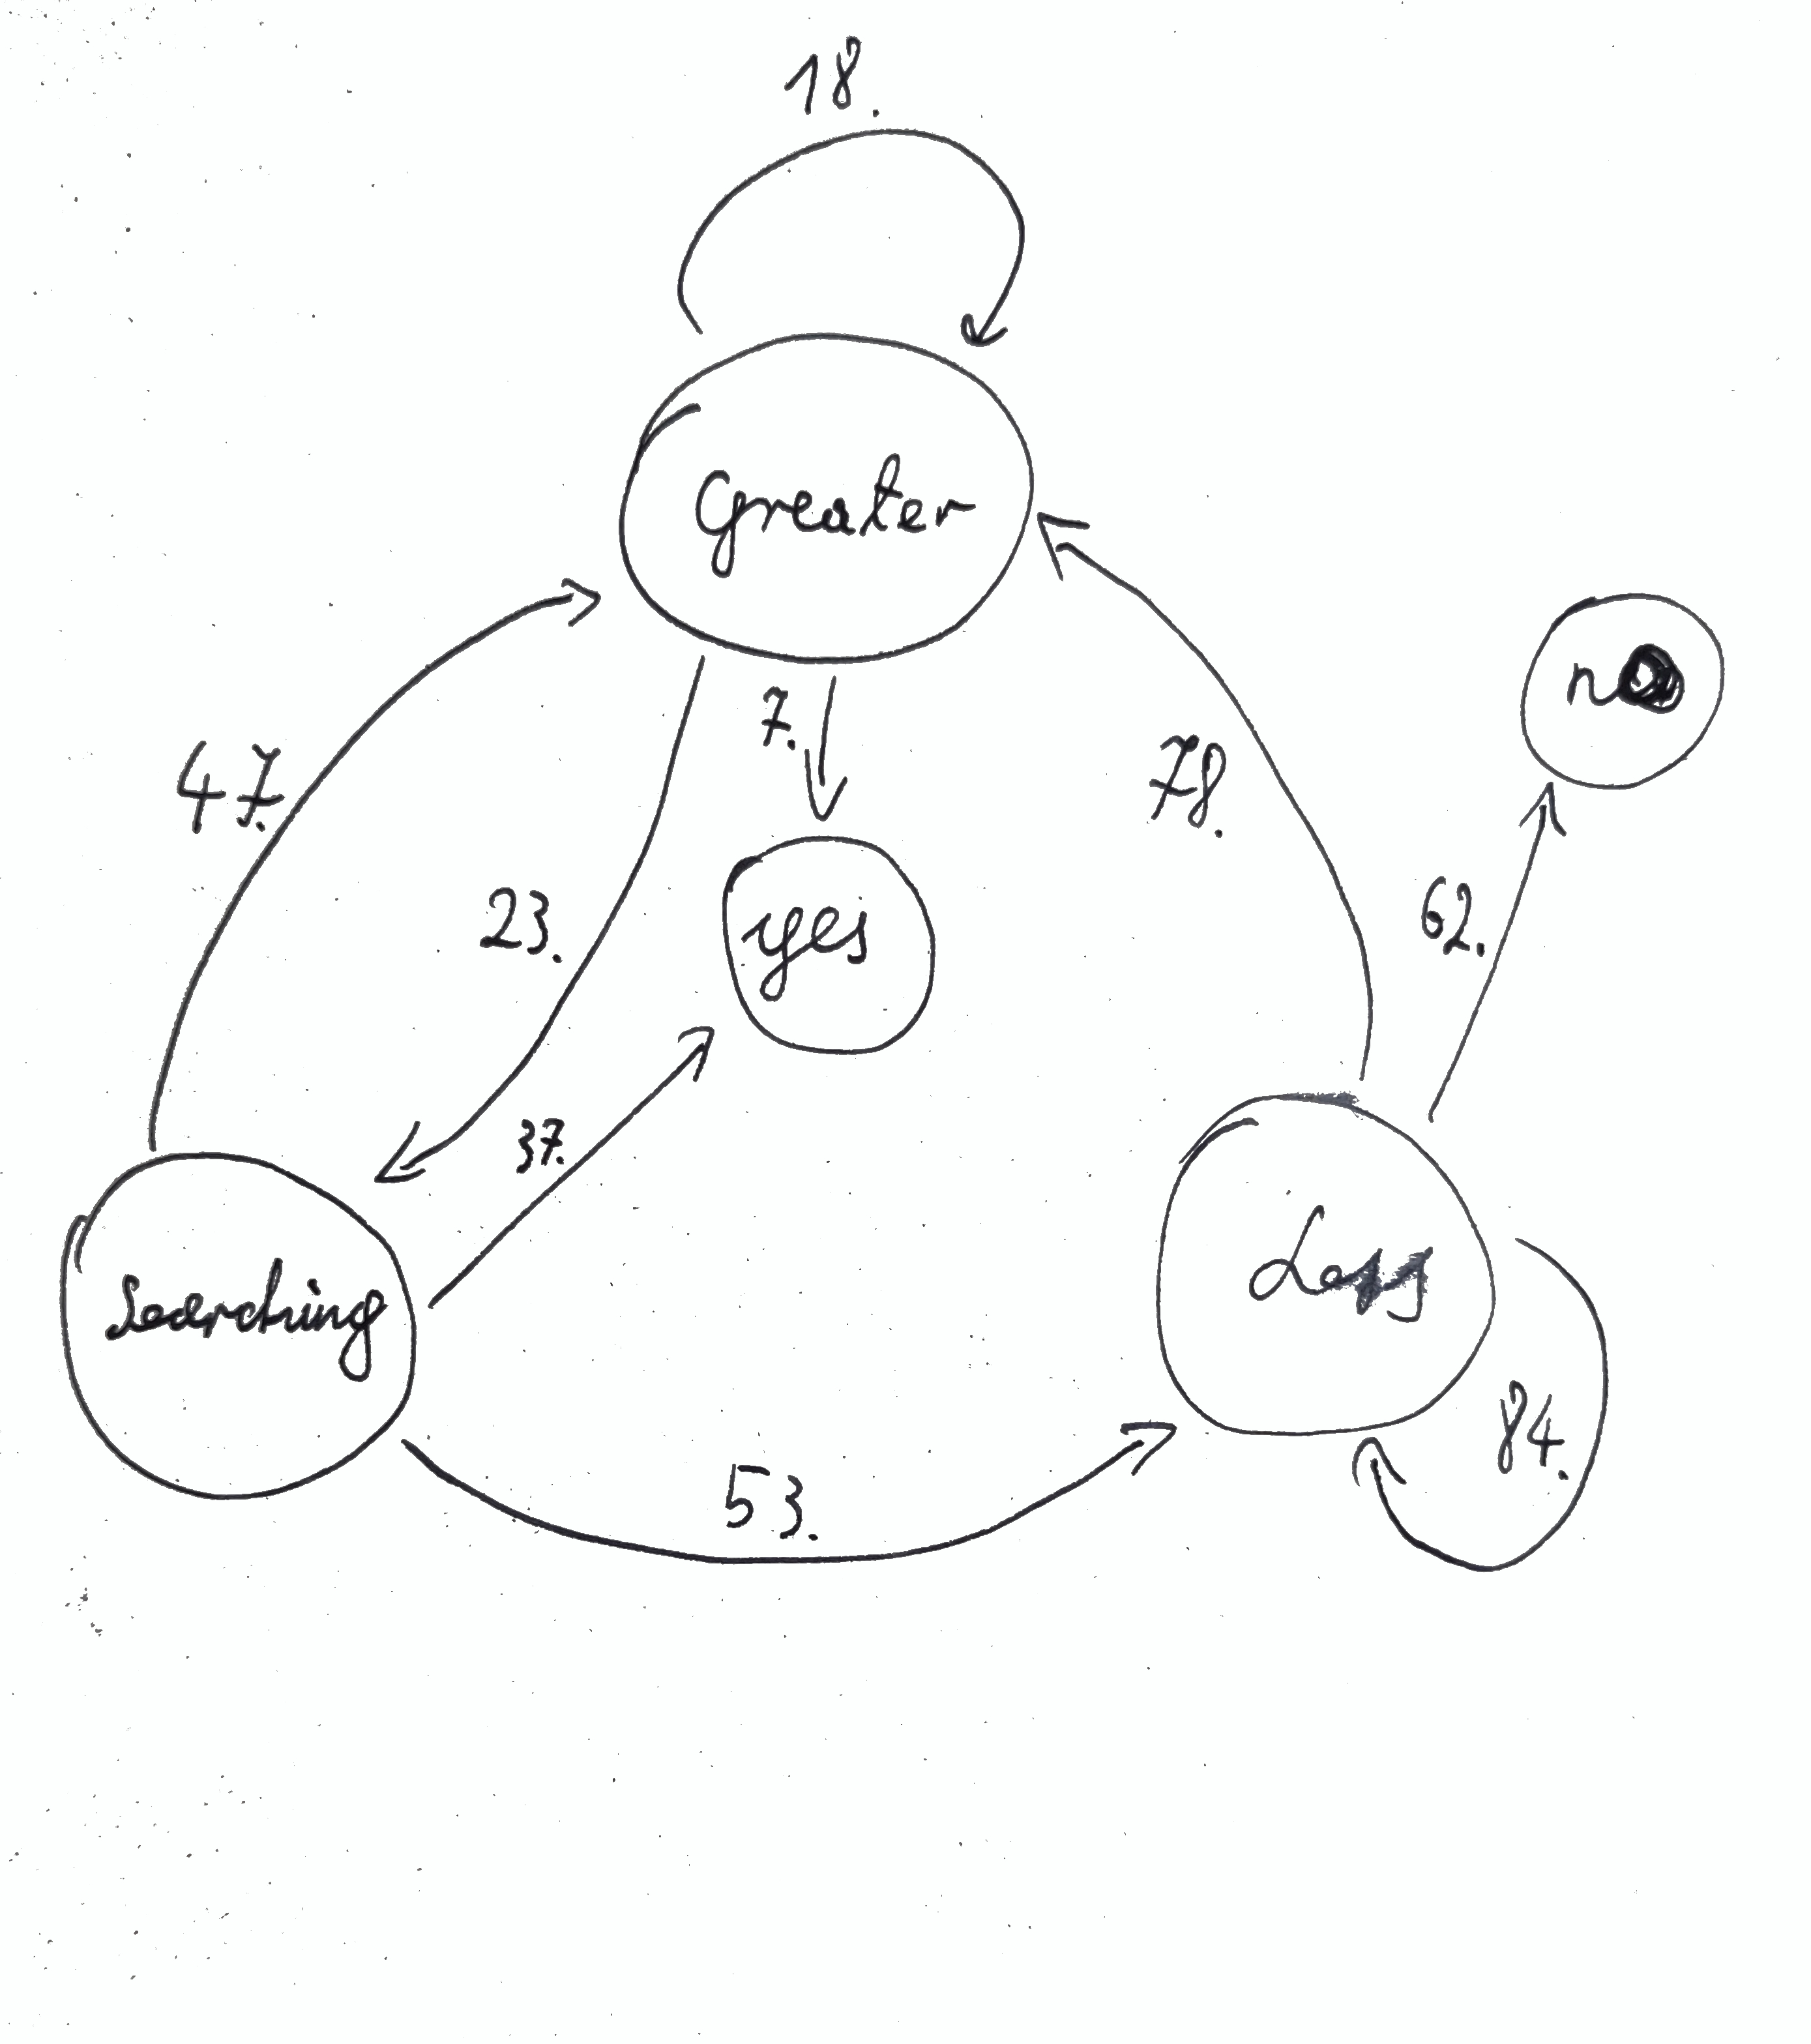
\includegraphics[width=\textwidth]{"../searching_for_a_spectrum/control_flow.jpg"}
\caption{Diagram of the control flow of the algorithm. Numbers above arrow indicate lines.}
\end{figure}
The execution of the algorithm then goes as follows:

We start at "Greater" and proceed to do the procedure from \ref{greater idea}. 
Once the procedure stops, we do procedure from \ref{searching mode idea}, then 
dependent whether the result have corresponding \Eoc\ greater or smaller than $\frac{p}{q}$, 
we perform, respectively -- again procedure from \ref{greater idea} or the 
procedure from \ref{less idea}. We repeat \ref{less idea} as long as necessarily. 
Once it gives the state that have \Eoc\ greater than $\frac{p}{q}$ we set the flag to 
"Greater" again and repeat the whole process starting from the procedure in \ref{greater idea}. 
In the case that repeating the procedure from \ref{Less idea} won't give any state with 
corresponding \Eoc\ greater than $\frac{p}{q}$ the algorithm will hit its stopping condition 
and answer "no" as written in the algorithm 
\ref{the algorithm for searching the spectrum itself} itself.   
% for searching the spectrum, that is
\section{Proof of the correctness of the algorithm}\label{memory state proof}
\subsection{Lemmas}\label{lemmas for the proof of the correctness}
Firstly, we will prove that our invariants indeed are conserved during the execution 
of the algorithm. We will also proof some other lemmas regarding the state of memory 
during the algorithm.

%-- THere are only finitely many couters non 1
\begin{lemma}
During any time of the execution of the algorithm, there are only finitely many counters 
that have non-$1$ value.
\end{lemma}
\subsubsection{Proof.}
We start with the state that have only finitely many non-$1$ value. Let us observe, that 
all three of the places -- lines: 15, 33-34, 64-65, 
where the counters are changed, change them in the way 
that preserves this state. As during any time of execution, there were only finitely many 
changes, we have the thesis. $_\square$

\begin{lemma}\label{Greater infinities to the left lemma}
When control is at the line 15. and the pivot is at the counter $c_p$, all counters 
to the left of $c_n$ are set to $\infty$. 
\end{lemma}
\subsubsection{Proof.}
We can get to the line 15th only in two ways: from line 18 in "Greater" section or from line 47 
in "Searching" section. 
In this process "Searching" moves pivot to the first counter and  
"Greater" moves pivot one counter to the right. 
As long as the pivot is not on the 1st counter, control flow must have came then to the line 15th 
from "Greater" section and if pivot is at the 1st counter it must have came from the 
"Searching" section. From this we have,  
that for the pivot, to get to the counter $c_p$, it would need to go through all 
the counters to the left of $c_p$ while being on the line 15th and 
setting them to $\infty$. 
\begin{lemma}\label{Searching infinities to the left lemma}
When control is at the line 33rd and the pivot is then at the counter $c_p$, all counters 
to the left of $c_p$ are set to $\infty$ and the counter $c_p$ is not set to $\infty$. 
\end{lemma}
\subsubsection{Proof.}
The only way to get to the line 33rd is from line 23rd in "Greater" section. 
From \ref{Greater infinities to the left lemma} we know, that then all the counters to the left 
of $c_p$ are set to $\infty$. Counter $c_p$ on the other hand can not be set to infinity, 
since, from the fact that control flow was at the block from line 21st, we know that
\begin{equation}
\cho{*d_1d_2\cdots d_{p-1}\infty d_{p+1}\cdots} < \frac{p}{q}
\end{equation}
and from the fact, that control flow was in the "Greater" block we know, that 
\begin{equation}
\cho{*d_1d_2d_3\cdots } > \frac{p}{q}._\square
\end{equation}

\begin{lemma}\label{state is ordered}
For any state of counters during the execution of the algorithm $D = d_1d_2d_3\cdots$ we have that 
$d_1 \geq d_2\geq d_3 \geq \cdots$.
\end{lemma}
%--order of counters is always decreasing
\subsubsection{Proof.}
We start with the state where $d_1 \geq d_2\geq d_3 \geq \cdots$. Let us observe, that, by 
\ref{Greater infinities to the left lemma}, changing at line 15 preserves this state. 
Changing at lines 33-34 or 64-65, preserve this state as they increase
the value of the counter at which pivot is by one (to some $d_p+1$) and change all counters 
to the left of the pivot to $d_p+1$. $_\square$

\begin{lemma}\label{Less same to the left lemma}
When control is at the line 66th and the pivot is then at the counter $c_p$, all counters 
to the left of $c_p$, are set to the same value $d_{p-1}$ and the counter $c_p$ 
is not set to the value $d_{p-1}$. 
\end{lemma}
\subsubsection{Proof.}
The only way for the control flow to get to the line 66th is from line 53th or 84th. 
In both of these cases, the counters to the left of $c_p$ were set to the same value on, 
respectively lines 33-34 or 64-65. Also, on lines 33-34 or 64-65, the value 
of the counter $c_{p-1}$ was increased by $1$. From this and 
from \ref{state is ordered}, we know, that $d_{p-1} > d_p$ 
%when we are at the line 66th
.$_\square$

\begin{lemma}\label{same value on the counters to the left}
All counters strictly to the left to the pivot have the same value 
%and 
%counter at the pivot have different value than these ones 
%at any of above lines. 
 at any stage of 
the execution of the algorithm.
\end{lemma}
\subsubsection{Proof.}
As state of the counters changes only on lines 15, 33-34 or 64-65, and 
the pivot is moving at most by one position to the right 
between the changes to the state of the counters, this is the 
corollary from \ref{Greater infinities to the left lemma}, 
\ref{Searching infinities to the left lemma} and \ref{Less same to the left lemma}. $_\square$

\begin{lemma}\label{Small searching always terminates}
Searching procedure from lines 29-32 always terminates.
\end{lemma}
\subsubsection{Proof.}
Let $c_p$ be the counter at which pivot is, when the searching procedure from lines 
29-32 stars. Control flow can get to the lines 29-32 only from line 23rd. This guarantees, that 
when starting the searching procedure, we have that:
\begin{equation}
\cho{*d_1d_2\cdots d_{p-1}\infty d_{p+1}\cdots} < \frac{p}{q}
\end{equation}
and  
\begin{equation}
\cho{*d_1d_2d_3\cdots } > \frac{p}{q}.
\end{equation}
From this and from \ref{chi supp functoriality non finite}, 
we know, that there exists some $d_p' < \infty$ such that 
\begin{equation}
\cho{*d_1d_2\cdots d_{p-1}d_p' d_{p+1}\cdots} < \frac{p}{q}
\end{equation}
As such, the searching procedure stops. $_\square$
\begin{lemma}\label{finitely many steps between counter changes}
There are always only finitely many steps in execution of the algorithm before it 
changes the state of the counters. 
\end{lemma}
\subsubsection{Proof.}
The only steps not explicitly listed in the algorithm are from the searching procedure from lines 
29-32. From \ref{Small searching always terminates} we know, that this procedure 
always terminates. 
All other control flow can be check explicitly to have always only finitely many steps between 
the change of the counters. 
The change of the counters itself is also a finite procedure, as we are always only changing 
the counters at pivot or at and to the left of the pivot, and there are only finitely many 
such counters. $_\square$
\begin{lemma}\label{always increases}
For any state $D_1$ that is a state of counters at some point of the execution of the algorithm 
and $D_2$ such that $D_1$ is changed to $D_2$ during the execution, we have that $D_1 \prec D_2$.
\end{lemma}
\subsubsection{Proof.}
Let us observe that in each instance of changing the counters -- in lines 15, 33-34 and 64-65. 
the rightmost counter that is changed is always increased. From this, the lemma follows. 
$_\square$
\subsection{Proof.}\label{proof of the correctness of the algorithm}
Now, we will perform the proof, that the idea of the algorithm presented above in 
\ref{the idea of the algoritm}, as 
well as the algorithm itself \ref{the algorithm for searching the spectrum itself}, 
works as intended.

Firstly, let us observe, that algorithm gives the answer only on lines 7-8, 37-38, 62, 68-69 and 
always ends immediately after giving the answer. Thus, it will always give at most one answer.
Furthermore let us observe that these are the only places where the algorithm terminates, 
so if it terminates it will give at least one answer.
 
There are three things to be checked: \\
$\bullet$ That the algorithm never answers "yes" if there is no orbifold of the \Eoc\ 
$\frac{p}{q}$ (No false positives)\\
$\bullet$ That the algorithm never answers "no" if there is an orbifold of \Eoc\ 
$\frac{p}{q}$ (No false negatives)\\ 
$\bullet$ That the algorithm always ends in a finite number of steps (Guaranteed termination). 

%To do this, we will introduce an order on the states of counters satisfying 
%\ref{valid state of counters}:



%\begin{lemma}

%\end{lemma}
%\subsubsection{Proof.}

%\begin{lemma}

%\end{lemma}
%\subsubsection{Proof.}

\subsection{No false positives}
Algorithm gives answer "yes" at lines 7-8, 37-38, 68-69. At each of these places, 
the answer contains the example of an orbifold with \Eoc\ equal to $\frac{p}{q}$ that was 
explicitly checked for correctness just before giving the answer (see lines 5, 35, 66). 
%$_\square$    
\subsection{No false negatives}
Let $D = d_1d_2d_3\cdots$ be such that $\cho{*d_1d_2d_3\cdots} = \frac{p}{q}$. 

%Let us assume for a contradiction, that algorithm started with $\frac{p}{q}$ answered "no". 
%
%We will show that this is impossible, by showing, that the algorithm will never 
%go beyond $d_1d_2\cdots$ in $\preceq$ order. 

First, we will show that the algorithm will never 
go beyond $d_1d_2d_3\cdots$ counter state in $\preceq$ order. 

Let us observe that the only lines where 
the counters are changed are lines 15, 33-34 and 64-65, 

Right before 
the change from 15 and right after each change from 33-34, 64-65 
(lines, respectively 5, 35, 66), 
the new state is checked if it is a solution and 
if it is a solution, the algorithm stops. From this, we 
have that going beyond $d_1d_2d_3\cdots$ can not happen from $d_1d_2d_3\cdots$, 
it must happen from some state $D' \preceq d_1d_2d_3\cdots$.

Furthermore while changing, 
only counters 
at pivot and to the left of the pivot are changed. 

Because of that:
\begin{observation}\label{position of pointer observation}
Going beyond $d_1d_2d_3\cdots$ counter state 
could happen only in lines 15, 33-34 or 64-65, while pivot would be 
%lovely
at the rightmost counter that is different from $d_1d_2d_3\cdots$ or further to the right. 
That is, if $d_1'd_2'd_3'\cdots$ is the current state, and 
$c_k$ is the rightmost counter on which $d_1d_2d_3\cdots$ 
and $d_1'd_2'd_3'\cdots$ differ and $c_n$ is the counter at which the pivot is on then 
at the moment of change that goes beyond $d_1d_2d_3\cdots$, it must hold that $k \leq n$.
\end{observation}
%This is because these are the only lines where the counters are changed and while changing, 
%only counters 
%at pivot and to the left of the pivot are changed. 

We will show that if the counters are below $D$ in $\preceq$ before the change they still 
be below $D$ or at $D$ after the change. 

We will now eliminate all three options arising from lines 15, 33-34 and 64-65 case by case. 
Let $D' = d_1'd_2'd_3'\cdots$ be current state of counters before the change 
during the execution of the algorithm. 
Let $c_k$ be the rightmost counter on which $d_1d_2d_3\cdots$ 
and $d_1'd_2'd_3'\cdots$ differ. Let $c_n$ be the counter at which the pivot is on. 
\subsubsection{Line 15}
%For the sake of contradiction, let us assume, that 
We will show that under taken assumptions, we will not get to this line. 
First, let us prove, that the pivot must be exactly at the counter $c_k$. 
By \ref{Greater infinities to the left lemma} we know, that if the pivot is 
on the counter $c_n$, while execution is at line 15, 
all the counters to the left of $c_n$ are set to $\infty$. 

This however means, that
\begin{equation}
\underbrace{\infty\infty\cdots\infty}_{n-1\ \mathrm{times}}d_nd{n+1}d_{n+2}\cdots \preceq D.
\end{equation}
Together with the fact, that for $k$, which is $\leq n$, we have that 
for any $l > k$, we have that $d_l = d_l'$ this means that if $n \geq k+1$, we have that 
$D = D'$. This is a contradiction with the assumption of $k$. 
From this we have that $n = k$.

We have then that pivot is on the rightmost counter $c_k$, 
that differs between $D$ and $D'$, and 
that all the counters strictly to the left of $c_k$ in $D'$ are set to $\infty$. 

%From the assumption that $D' \preceq D$ we know, that $d_k' < d_k$. 

From this, since $\cho{*d_1d_2d_3\cdots} = \frac{p}{q}$, we have, that: 
\begin{equation}
\cho{*d_1'd_2'd_3'\cdots d_{k-1}'\infty d_{k+1}'\cdots} \leq \frac{p}{q} 
\end{equation}

From this, we have the contradiction with the assumption that we will get to the line 15. 

\subsubsection{Lines 33-34}
Similarly as in the previous case, this time using \ref{Searching infinities to the left lemma} 
we can prove, that $n=k$, as well as that $d_k' < d_k$, that all 
counters strictly to the left of $c_k$ in $D'$ also must be $\infty$.

This leads us to the conclusion that searching procedure from lines 
29-32 will find some $ d_k'' \leq d_k$ as a result. Then, the resulting state 
still will be $\preceq D$. 

\subsubsection{Lines 64-65}
We will show the contradiction by showing that pivot must be on 
the counter strictly to the left of $c_k$. 
%We will show that $n = k$. 
By \ref{Less same to the left lemma} 
we know, that all the counters to the left of $c_n$ are set to $d_{n-1}'$. 
From this, from the fact that $d_k' < d_k$ and 
from the fact that $\cho{*d_1d_2d_3\cdots} = \frac{p}{q}$, 
we have that, unless $n < k$, we have that 
\begin{equation}
\cho{*d_1'd_2'd_3'\cdots} \geq \frac{p}{q}.
\end{equation}
However, this is a contradiction with being at lines 64-65, as 
the only way to get there with the execution, is either from lines 
51-53 or the lines 82-84, reaching either require for the state of counters to have 
corresponding \Eoc\ $<\frac{p}{q}$.

% We can get to line 64 only if the configuration (all of the pivot to 
%the left the same ) ha \Eoc smaller thsn pq. However, this has no smaller . 

\subsection{Guaranteed termination}
First let us observe, that 
Let 
\begin{equation}
_\infty D = \underbrace{\infty\ \infty\ \infty\cdots 
\infty\ }_{\lfloor 2(1-\frac{p}{q})\rfloor\ \mathrm{times}}1\ 1\ 1\cdots
\end{equation}
and let 
\begin{equation}
_2D = \underbrace{2\ 2\ 2\cdots 
2\ }_{\lceil 4(1-\frac{p}{q})\rceil\ \mathrm{times}}1\ 1\ 1\cdots.
\end{equation}
These are the state consisting of only, respectively, $\infty$ and $2$ as a non-$1$ counters 
values, that have the property, that they have the most non-$1$ counters from all 
states of such form, having the corresponding \Eoc\ $\geq\frac{p}{q}$. 

Let us assume that for some input $M$ and $\frac{p}{q}$ the algorithm does not answer "yes". 
We will show, that then it will answer "no" in finite number of steps. By 
\ref{finitely many steps between counter changes} 
we can show this, by showing, that it will answer "no" after 
finitely many of counters state changes. 
\subsubsection{Going beyond every state smaller or equal than $_2D$}\label{going beyond}
We will show it by firstly showing, that for any state $D = d_1d_2d_3\cdots$ smaller 
or equal to  
$D_2$ the algorithm will go to it or beyond it.
%\begin{enumerate}
%    \item if the pivot is on the zeroth column ($c = 0$), then 
%    \begin{enumerate}[label*=\arabic*.]
%        \item 
%        \item
%    \end{enumerate}
%    \item abcd
%\end{enumerate}
%\section{Improvements}
%We will prove that for any state different than 222222 it will go beyond it.

Proof will be inductive, with respect to order $\preceq$. Our inductive assumption will be, that 
for a given state $D$, that is at most $D_2$, 
%all the states $D'\prec D$ 
%have 
there is some state $D'$, such 
that $D\preceq D''$, and that $D'$ was the state of the counters after a finite 
number of steps of execution of the algorithm. 
%at some point. 

$\bullet$ For the fist state we have that this is true since it is the $D'$ for itself.
%for all the previous ones.   

$\bullet$ Let us suppose that for a state $D = d_1d_2d_3\cdots \preceq D_2$, for  
all the states $\prec D$ our inductive assumption holds. We will show that it holds 
for $D$. 
 
We will have two cases. 
\begin{itemize}
\item $D$ is a successor of some $D_1$. 
There are two options -- either $D_1$ was a state of counters 
at some point of the execution, or it wasn't. 

If it wasn't, from the inductive assumption we know 
that some state equal at least $D$ was the state of counters. From this we have the induction 
thesis for $D$.

In the case $D_1$ was a state of counters, from \ref{always increases} we have, that the next 
state of counters will be equal at least $D$.  
%there are three cases
%, depending on 
%which lines will be the change from $D_1$ to the next state in the execution. 
%\begin{itemize}
%\item Line 15 

%in this case the state is chenged 
%\item Line 


%\item Line

% 
%\end{itemize}
%here there will be 222222 as an exeption


\item $D$ is not a successor of any $D' \prec D$. From this, we have that $D$ has at least one 
$\infty$ on its counters.  
Let $c_l$ be the counter that has rightmost infinity in $D$. 
From \ref{} we have, that all the counters to the left of $c_l$ also are set to $\infty$.

Let us consider the state $^0D = ^0d_1^0d_2^0d_3'\cdots$, such that for any $i > l$, we have that 
$^0d_i = d_i$. From the induction assumption, there exists state $D' = d_1'd_2'd_3'\cdots$ 
such that $^0D\preceq D'$ and such that $D'$ was a state of the counters after finitely 
many steps of the algorithm. If $D' \succeq D$, then we have induction thesis for $D$. 
Let us consider the case, where $D' \prec D$. Then, since $^0D \preceq D' \prec D$, we have 
that for every $i > l$, we have $d_i' = d_i$. From this, we have, that $D'$ differs from 
$D$ only on the counters at, or to the left of $c_l$. We know, that all the counters 
to the left of, or at $c_l$
are set to $\infty$ in $D$ and that there is at least one counter set to $\infty$. 
Moreover, we know, that $D'$ differ from $D$ on at least one counter.

There are two cases:
\begin{itemize}
\item $\cho{D} \geq \frac{p}{q}$ 
From this, we conclude 
that $\cho{D'} > \frac{p}{q}$. 

Regardless of at which line state $D'$ was produced, the execution will then follow, 
through line  or to the line    . From this point, since $\cho{D} \geq \frac{p}{q}$, we will 
have consecutive sequence length at most $l$, of states of counters, where 
values of consecutive counters 
from $D'$ will be 
replaced by $\infty$, up to the counter $c_l$ at which state $D$ will be reached. 
This sequence will be generated by repeatedly going through line 15 in the algorithm, since 
at every step, the corresponding \Eoc of the state of counters will be $> \frac{p}{q}$.

\item $\cho{D} < \frac{p}{q}$
From \ref{chi supp functoriality non finite}, we know, that there must exists state 
\begin{equation}^0D = ^0d_1^0d_2^0d_3'\cdots,
\end{equation} 
such that 
all $^0d_i$ are less than $\infty$ and are the same for 
any $i \leq l$, and that $\cho{^0D} < \frac{p}{q}$. 

From this, we conclude, that $\cho{D'} < \frac{p}{q}$. 
Regardless of at which line state $D'$ was produced, the execution will then follow, 
through line 53 or 84 to the lines 64-65. From this point, since $\cho{D'} < \frac{p}{q}$, 
we will 
have consecutive sequence length at most $l$, of states of counters, where 
values of consecutive counters 
from $D'$ will be increased by one and all the counters to the left of them will be set to 
the value of the counter which was just increased. 
This sequence will be generated by repeatedly going through lines 64-65 in the algorithm, since 
at every step, the corresponding \Eoc of the state of counters will be $< \frac{p}{q}$.

This sequence will end by going with the pivot to the counter $c_{l+1}$, which we 
know from the assumption that has value smaller than $\infty$, increasing it by one 
and setting all the counters to the left of if to value $d_{l+1}+1$, this way obtaining 
the state larger in $\preceq$ than $D$. 
\end{itemize}

%From the inductive assumption, we know that for any state $D' \preceq D$.
%Let us take an ascending sequence of ${D_n}$, such that   
%Let take the smallest ones for each. if any of them 
%are greater than D we are done, so let us suppouse that they are all smaller. 

%This needs to be a finite set, since there was only finitely many states as a stets of counters. 
%This means that, since for every non infty one there are some ddadada there is an upper limit 
%dadada. THere is one that has $infty$ at this . Since they have the same to the right as D 
%it must be 
%greater or equal than D,  
\end{itemize}
\subsubsection{Reaching $_2D$ at finite number of steps}
Now we will show that at some point, algorithm will have as a state of counters $_2D$. 

\begin{lemma}\label{incorporating counters}
Every counter with number greater than $\lfloor 2(1-\frac{p}{q})\rfloor\ \mathrm{times}$ 
has pivot on it for the first time while the execution is in line 
\end{lemma}
%Let us observe that 
\subsubsection{Proof.}


From this, we have, that every time there is a state of counters that for the first time 
involves counter with number greater than 
$\lfloor 2(1-\frac{p}{q})\rfloor\ \mathrm{times}$, it is the state 
of the form $2\ 2\ 2\cdots\ 2\ 1\ 1\ 1\cdots$. 
Since from \ref{going beyond} 
we know that for every state $D \preceq _2D$, 
we will have some bigger state $D'$, that at some point was a state of counters, we 
have that at some point counter $c_{\lceil 4(1-\frac{p}{q})\rceil}$ will 
obtain non-zero value (if the predecessor of $_2 D$ will be the state of counters 
at some point, then $c_{\lceil 4(1-\frac{p}{q})\rceil}$ will have non-$1$ value at the 
next change of counters.). 
%We have 
%some state $_\infty D' \succeq _\infty D$. In the next change of the conters, state of 
%the counters will have non-$1$ value at the counter $\lfloor 2(1-\frac{p}{q})\rfloor + 1$.
From \ref{incorporating counters}, we know, that then there must have been state $_2D$ 
at some point as a state of counters. 
%The smallest biggest state involves additiona lcounter 
%and by what we shouwed then there will be 222222. 
$_\square$





\section{Another questions the algorithm can answer}
\subsection{Deciding the order of accumulation}
Using above algorithm, for a point $\frac{p}{q}$ and a manifold $M$, we can check 
what order of accumulation point $\frac{p}{q}$ is in $\spebr{M}$. 

Analogously to \ref{algorithm reduction to D2}, we will wlog answer the question fr $ M = D^2$. 

First, we check with the algorithm, whether $\frac{p}{q} \in \speD$. If not, it is not 
an accumulation point of $\speD$, since \ref{accumulation_points_of_the_set}.

Let us now consider the case, where $\frac{p}{q} \in \speD$.

From \ref{predescors}, we know, that for a point $\frac{p}{q}$ being an accumulation 
point of the set $\speD$, of order at least $n$ is equivalent to the fact that 
$\frac{p}{q} + \frac{n}{2} \in \speD$. From \ref{spectrum lesser than chi} 
on the other hand, we know, that 
for any $x > 1$, we have $x \not\in \speD$.

%Let us assume, that $\frac{p}{q} \in D^2$
  
As such, for a given $\frac{p}{q}$, we can, using our algorithm, check one by one 
every number of the form $\frac{p}{q} + \frac{n}{2}$, such that $n \in \mathbb{N}_0$ and 
$\frac{p}{q} + \frac{n}{2} < 1$. There are at most 
$\lfloor 2 \left(1 -\frac{p}{q} \right)\rfloor$ such numbers. 
Let $n_0$, be the biggest of the checked numbers, for which 
$\frac{p}{q} + \frac{n}{2} \in \speD$. 
Then, from \ref{predescors} 
we know, that $\frac{p}{q}$ is an accumulation point of order $n_0$ in $\speD$. 

 

%\todo{poprawić}
%Let $m \in \mathbb{N}$ be such that $\frac{p}{q} \in (1-\frac{m}{2},1-
%\frac{m+1}{2})$
%Let us denote by $r \coloneqq \frac{p}{q} - (1-\frac{m}{2})$. \\ 

%We will searching in $\sigma$ as such: \\

%If $\frac{p}{q} \in \sigma$, then, from the corollary \ref{predescors} we know, that there 
%exist some $n \in \mathbb{N}$, such that $\frac{p}{q} + \frac{n}{2} \in \sigma$ but 
%$\frac{p}{q} + \frac{n}{2} \not\in \sigma$. \\

%We will be consequently checking points from $1+r$, through $1+r-\frac{l}{2}$, for 
%$0 \leq l \leq m$, to the $\frac{p}{q}$. We stop at the first found point. 
%If one of these point is in the spectrum, then all smaller (so also $\frac{p}{q}$) are in 
%the spectrum and $\frac{p}{q}$ is the accumulation point of the spectrum of order $m-l$ 
%(from this, 
%we can see some heuristic, that the points that have smaller order will be generally 
%harder to find in some sense). If none of this points are in in the spectrum, then $\frac{p}{q}$ 
%is not. \\

\section{Implementation}
This algorithm is a part of the algorithm from chapter \ref{Counting orbifolds -- arithmetical part} 
where the implementation of the whole will be discussed in \ref{implementation}.
